\section{Descrição da Planta}
\begin{figure}
    \centering 
    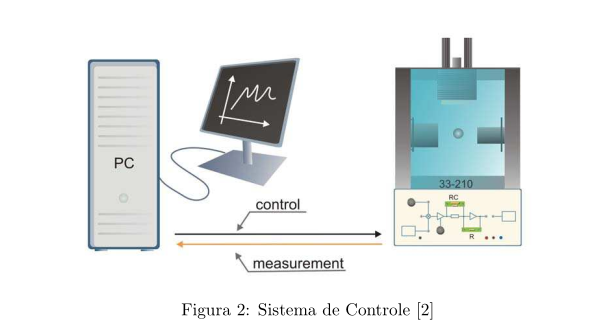
\includegraphics[width=\linewidth]{control.png}
    \caption{ Sistema de Controle [1]}
    \label{fig:2}
\end{figure}
A planta utilizada para estudo é mostrada na Figura 2. O sistema apresentado funciona da seguinte forma:

\begin{itemize}
    \item Um computador, equipado com uma placa de aquisição de dados da Advantech, funciona como unidade central de controle em conjunto com os ambientes MATLAB e Simulink. Os sinais de controle, variando entre -5V e 5V, são enviados ao módulo do levitador, que os converte em corrente elétrica aplicada à bobina, gerando o campo magnético responsável pela levitação.
    \item A posição da esfera magnética é detectada por um senosr infravermelho integrado à estrutura do sistema. Esses dados de posição são transmitidos ao computador por meio da interface de comunicação, onde os algoritmos de controle implementados pelo Simulink processam as informações e ajustam o sistema em tempo real.
\end{itemize}

\subsection{Variáveis do Processo}
\begin{description}
    \item[Variável Manipulada:] Tensão de controle aplicada ao Levitador Magnético.
    \item[Variável Medida:] Posição da esfera, medida pelo sensor infravermelho, convertida em sinal de tensão.
    \item[Variável de Referência:] Posição desejada esfera, set-point. 
\end{description}

\subsection{Sensores e Atuadores}
\begin{description}
    \item[Planta] A unidade mecânica do sistema de levitagão magnética.
    \item[Sensor] Sensor infravermelho usado para medir a posição vertical da esfera suspensa no ar.
    \item[Atuador] Circuito de controle que aplica a tensão ao núcleo magnético, gerando o campo magnético para levitar a esfera. 
\end{description}

\subsection{Pertubações e Não Linearidades}
\begin{description}
    \item[Pertubações] O sistema pode ser afetado por vibrações externas, variações na carga, que podem comprometer a estabilidade da esfera em levitação.
    \item[Não Linearidades] O sistema apresenta característica não linear devido à natureza da força de atração eletromagnética, que pode ser expressa pela seguinte equação: 
    \begin{equation}
        F_{M} = k \frac{i^{2}}{x^{2}}
        \label{eq: forca_magnetica}
    \end{equation}
    em que, $F_{M}$ representa a força magnética, $i$ é a corrente aplicada à bobina, $x$ é a distância vertical da esfera em relação ao sensor, e $k$ é uma constante do sistema.
\end{description}